
\chapter{Diskussion}
Im vorhergegangen Kapitel wurden die \gls{glos:onPremiseLabel} Lösung beschrieben, sowie das Auslagern der Workstations in die \Gls{glos:cloudLabel} auf fremden (\Gls{daasLabel}) und eigenen Servern (\Gls{vdiLabel}). In diesem Kapitel werden die verschiedenen Vorgehen gegeneinander verglichen. Das Kapitel soll helfen, sich für eine Lösung zu entscheiden.

% http://www.stratacore.com/blog/choosing-between-vdi-and-daas
% DaaS vs VDI
% + daas
	% Load balancing
	% Software and security updates
	% Installations
	% Network maintenance
	% Schneller aufgesetzt
	% better cost benefit / ROI
% + vdi
	% slightly faster, because local datacenter, no firewall
	% recommended when data security is top priority

\section{Vor- und Nachteile}
%sl
% sources:
% http://searchvirtualdesktop.techtarget.com/feature/DaaS-vs-VDI-comparison-highlights-benefits-of-cloud-desktops
% http://searchvirtualdesktop.techtarget.com/tip/Virtual-desktop-benefits-that-sell-VDI

% kosten abschätzbar
% günstiger für viele workstations
% günstiger da outsourcing möglich
% kosten abschätzbar
% thin clients günstiger

% Greater control how you secure your desktop
% e.g prevent users from copy files to local machine

% daas
% einfacher
% günstiger

Um \gls{glos:onPremiseLabel}, \Gls{daasLabel} und \Gls{vdiLabel} zu vergleichen müssen die Vor- und Nachteile analysiert werden.
Unterteilt wird die Diskussion in die Bereiche Kosten, Aufwand, Unterhalt und Sicherheit.

\subsection{Kosten}
%http://betanews.com/2013/11/04/comparing-cloud-vs-on-premise-six-hidden-costs-people-always-forget-about/
% costs can heavily depend!
% to calculate costs of on premis soly on new hard-/software is like judging a book by its cover
% Same for cloud. They only calculate montly costs
% What needs to be regarded in the calculation:
	% - Electricity costs. Powering and cooling. Costs hard to meassure. Ask google/facebook. They need to watch PUE (Power Usage Effectivness)
		% More important the bigger you get.
	% - Bandwidth: Server inhouse: only limitation is the network infastructure. Ask a trusted consultant on what bandwidth you need for the cloud.
		% Check http://bandwidthpool.com/ for what you need. Login required.
	% - Cloudserver outbound bandwidth: You pay as you requst data
		% You can load as many data on the server, but pulling them out costs bandwidth
		% Understandable, you save money by not hosting them by yourself
		% not a big problem for virtual desktops
	% - Five year rule: On average, you need to replace 24/7 servers every 5 years
		% Cost diagram: http://www.softwareadvice.com/tco/ for SaaS, but maps to DaaS.
		% DaaS, higher recuring costs. but no 5 year hit-backs
	% - Downtime costs: The more they costs, the more it worth going into the cloud
		% Downtime cost calculator: http://www.visionsolutions.com/Solutions/Disaster-Recovery-toolkit-downtime-calc.aspx
		% Accross USA & EU, each year  $26.5 Billion USD is lost because of IT downtime

Im \cref{sec:vmwareCosts} wurde aufgezeigt, dass es kostspielig sein kann, auf eine \Gls{vdiLabel}-Lösung umzustellen. Es müssen deshalb konkrete Bedürfnisse vorhanden sein, damit sich eine Umstellung rechtfertigt.

Bei der Berechnung der Kosten wird oft der Fehler gemacht, dass nur die Hard- und Software Kosten bei \gls{glos:onPremiseLabel} und \Gls{vdiLabel} berücksichtigt werden, und die monatlichen Kosten bei \Gls{daasLabel}.
Dass ist jedoch das selbe, wie wenn ein Buch nur nach dessen Deckblatt bewertet wird.
Es gibt diverse andere Kosten die es zu beachten gilt.

\subsubsection{Strom}
Kosten welche oft nicht berücksichtigt werden sind jene für die Elektrizität.
% von hier...
Diese können unterteilt werden in die für den Stromverbrauch der Geräten, sowie in die Stromkosten, welche durch die Kühlung anfallen.
% ... bis hier evt löschen?

Je grösser die Firma wird, desto grösser wird dementsprechend auch der Stromverbrauch. Dies wird noch verstärkt oder abgeschwächt nach dem Arbeitsgebiet auf dem das Geschäft operiert. Bei einem Service-orientiertem Angebot ist der Konsum deutlich höher.

Unter den gesamten Ausgaben für die Elektrizität sind die Kosten für die Server oft schwer raus zu lesen, wenn keine Messwerkzeuge installiert sind. Der Vorteil von einem externen Anbieter besteht darin, dass diese Kosten bereits in den monatlichen Umtrieben enthalten sind.

Im Vergleich von \gls{glos:onPremiseLabel} und \Gls{vdiLabel} hat sich in der Erfahrung gezeigt, dass die Stromkosten sich nicht merklich unterscheiden. Bei \Gls{vdiLabel} konsumieren die Server mehr Strom. Da die Mitarbeiter jedoch nur noch leistungsschwache Rechner benötigen, die sich auf die Desktops auf den Servern verbinden, benötigen diese weniger Strom. Dies hebt sich gegenseitig auf.

Um die Effektivität des Stromverbrauches eines Datencenters zu messen gibt es das \Gls{pueLabel} Verhältnis. Dazu wird der gesamte Verbrauch einer Firma geteilt durch Stromkosten der IT gerechnet.
\[\text{PUE} = \frac{\text{Total Stromkosten}}{\text{Stromkosten der IT}}\]
Je näher der Wert bei 1 liegt, desto besser ist er. Microsoft gibt an, einen \Gls{pueLabel} Wert zwischen 1.13 bis 1.2 zu besitzen und Google arbeitet mit 1.14.

Den \Gls{pueLabel} Wert auf ein erträgliches Mass zu reduzieren kann zum Teil schwierig oder kostspielig sein, wenn man seine ganze Infrastruktur umstellen muss. Eine \Gls{glos:cloudLabel}-Lösung stellt ein geeignetes Mittel dazu dar.

\subsubsection{Datenraten}
Ein weiterer Kostenpunkt sind die Datenraten und Netzwerkkosten. Bei einer \Gls{daasLabel} können beträchtliche Datenraten anfallen, wenn Dateien, Programme und weiteres ausser Haus gespeichert werden. Wenn jedoch nur der Bildschirm übertragen wird halten sich die Kosten in Grenzen. Bei dem Betreiben der Server in-house fallen zwar keine Internet kosten an, jedoch wird das eigene Netzwerk stark belastet.

Für eine neue Firma ist es meist günstiger von Anfang an, in der \Gls{glos:cloudLabel} zu arbeiten, da keine Kosten für das Aufziehen eines Netzwerkes anfallen.
Hat man hingegen bereits ein bestehendes, gut ausgebautes Netzwerk, kann dies eine Hürde darstellen beim Umstieg in die \Gls{glos:cloudLabel}.

Zur Berechnung der benötigten Datenraten gibt es Berechnungssoftware oder auch online Services zu finden. Ein Beispiel ist Bandwidth Pool \footcite{What_is_Bandwidth_Pool_Bandwidth_Pool}.

Ein versteckter Kostenpunkt bei gewiesen Clouddiensten sind die auswärts Datenraten. Man kann gratis und so viele Daten man möchte auf einen Server laden, diese anschliessend ab zugreifen kostet.
Auch diese Kosten sind für \Gls{daasLabel} Lösungen nicht sehr hoch, müssen jedoch mit eingerechnet werden.

\subsubsection{5-Jahre-Regel}
Im Durchschnitt müssen Hardware-Komponenten alle fünf Jahre ausgetauscht werden. Dabei handelt es sich um einen Richtwert, weshalb der tatsächliche Wert schwer abzuschätzen ist.

Wird die 5-Jahre-Regel nicht berücksichtigt, kann es dazu kommen, dass nur die initialen Kosten, sowie die Unterhaltskosten berücksichtigt werden.
Wenn der Anschein trügt und die Kosten mit der verzerrten Rechnung günstiger sind als die einer \Gls{glos:cloudLabel}-Lösung, kann sich dass nach fünf Jahren ändern, denn dann werden die Kosten steigen, weil alte Hardware ersetzt werden muss.

\begin{figure}[H]
	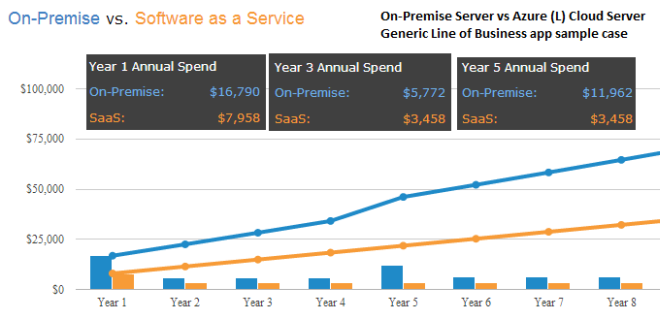
\includegraphics[width=0.8\textwidth]{images/five-year-rule}
	\caption{5-Jahre-Regel}
%	\source{\cite{Comparing_cloud_vs_on-premise_Six_hidden_costs_people_always_forget_about}}
	\label{fig:fiveYearRuleImage}
\end{figure}
% \footcite{Comparing_cloud_vs_on-premise_Six_hidden_costs_people_always_forget_about}
Die Graphik verdeutlicht, dass zwischen Jahr 4 und Jahr 5 der Preis ein Anstieg macht, da zusätzliche Hardware gekauft werden muss

Hier liegt der Vorteil von \Gls{daasLabel} darin, dass die Kosten klar definiert und in das Jahresbudget mit eingerechnet werden können.

\subsubsection{Ausfallkosten}
Bei \gls{glos:onPremiseLabel} und \Gls{vdiLabel} ist es kostenintensiv und kompliziert, eine hohe Ausfallsicherheit zu erreichen. Zum Beispiel muss ein \gls{glos:loadBalancingLabel} eingerichtet werden, sowie Daten- und Internetleitungen müssen redundant angelegt werden. Um diese Strategien erfolgreich umzusetzen, ist teures Expertenwissen nötig.

Bei externem Hosting mit \Gls{daasLabel} wird die Ausfallsicherheit extern für viele Benutzer verwaltet, wodurch Synergien genutzt und Kosten reduziert werden.

Für bestehende Firmen muss abgewogen werden, wie hoch die Kosten eines Ausfalles sind. Ist eine hohe Verfügbarkeit nötig, rechnet sich die Umstellung in die \Gls{glos:cloudLabel} schnell. Für eine einfache Berechnung der Ausfallkosten gibt es den Online-Rechner von VisionSolutions.\footcite{Disaster_Recovery_Resouce_Center_-_Vision_Solutions}

Hingegen für Startup Firma, bei der eine hohe Verfügbarkeit nötig ist wird empfohlen, früh auf Clouddienste zu setzen.

\subsubsection{Outsourcing}
Das Outsourcing des Supports zieht zwar weitere Umstellungen für die Firma mit sich, es kann, wie im Kapitel \cref{sec:vmwareCosts} ausführlich Diskutiert, jedoch sehr viel Geld eingespart werden. Dies rechnet sich mehr, je grösser der Betrieb ist.

Outsourcing kann für die \Gls{glos:cloudLabel} genau so betrieben werden wie für \gls{glos:onPremiseLabel} Lösungen. Jedoch hat der Support in der \Gls{glos:cloudLabel} und im spezielen bei \Gls{daasLabel} viel mehr Möglichkeiten auf die Desktops Einfluss zu nehmen. Stehen die Server in-house wird es immer ein grösseres Team an IT-Spezialisten in der Firma geben.

\subsubsection{Fazit}
Die Kosten sind schwierig zu berechnen. Es spielen viele Faktoren eine Rolle und die Übersicht zu bewahren ist schwierig.

Elektrizität-Kosten sind bei in-house Servern sehr hoch. Es sollte ein \Gls{pueLabel}-Wert zwischen 1.1 und 1.2 angestrebt werden. Alternativ lohnt sich ein Wechsel auf \Gls{daasLabel} um die Kosten auf den Sevice-Anbieter abzuwählen.

Datenraten spielen im Allgemeinen in der \Gls{glos:cloudLabel} eine grosse Rolle, wenn jedoch nur der Desktop übertragen wird halten sich die Datenvolumen in Grenzen. Hat man eine gut ausgebautes Netzwerk bietet es sich an, auf \Gls{vdiLabel} zu setzen um die bestehende Infrastruktur weiter zu nutzen.

Der grösste Kostenpunkt in der Rechnung der IT sind meist die Hardwarekosten. Deshalb ist es essenziell das man bei in-house Lösungen die 5-Jahre-Regel beachtet. Sind die Kosten mit Berücksichtigung der 5-Jahres-Regel günstiger als die einer \Gls{daasLabel}-Lösung, so sollte ein in-house Hosting betrieben werden. Entweder mit \gls{glos:onPremiseLabel} oder \Gls{vdiLabel}. Sonst sollte \Gls{daasLabel} eingesetzt werden.

Eine hohe Verfügbarkeit ist teuer wenn sie mit in-house System realisiert werden muss. Deshalb muss eine genaue Recherche betrieben werden wie teuer ein Ausfall wäre. Der Vorteil von \Gls{daasLabel} liegt darin, dass man sich nicht um die Verfügbarkeit kümmern muss und stellt deshalb eine günstige Variante dar um das Ziel zu erreichen.

Für grosse Firmen kann es luktrativ sein ein Teil der Arbeit zu Outsourcen. Verfügt man über \Gls{vdiLabel} oder DaaS ist es ein leichtes Externen Kontrolle über die \Gls{vdiLabel} oder \Gls{daasLabel} Umgebung zur Verfügung zu stellen. Stehen die Server in-house ist jedoch immer noch ein Team vor Ort nötig.

\subsection{Aufwände \& Unterhalt}


% pilots einfach
% incremental scaling
% Ein image für alle benutzer
% Updates einfacher. Eine Zentrale stelle für updates
	% Evt muss für updates neue hardware angeschaft werden. Mehr ram etc.
% Updates/Deployments sind lighning fast
% Fehler auffinden einfacher, da nur in einem system gesucht werden muss
% Backup an einer zentraler stelle

% Go green. Thin clients brauchen weniger strom
% Platform unabhängig. Egal ob windows, mac, linux
% Work from abroad
% Performance besser genutzt / Reductions in computing hardware needs.
% Improved workplace/user flexibility,

Die Aufwände sind unterteilt in Initiale- und Wartungsaufwände.

Die Initialen-Aufwände umfassen die Beschaffung und Einrichtung der Hardware sowie allfälliger Netzwerkerweiterungen. \Gls{daasLabel} hat den Vorteil das man nur \glspl{glos:thinClientLabel} angeschafft werden müssen. Hingegen muss bei VDI leistungs-starke Server und zusätzlich die \glspl{glos:thinClientLabel} eingekauft werden.

Im Unterhalt bieten die \Gls{glos:cloudLabel}-Lösungen die meisten Vorteile, da sie sehr flexibel sind. Es kann sehr einfach skaliert werden. Bei Bedarf kann auf Knopfdruck 10 neue, komplett eingerichtete,  Desktops erstellt werden. Es können Templates generiert werden, so dass eine Führungsperson eine andere Konfiguration erhalten als eine Sekretärin.

Updates und die Verteilung neuer Software können zentral verwaltet und innerhalb von Minuten auf alle Desktops verteilt werden. Es braucht keine klassischen Scripts mehr welche auf jedem Rechner einzeln ausgeführt werden müssen.

\gls{glos:homeOfficeLabel} wird mit der \Gls{glos:cloudLabel} vereinfacht. Es muss nur an einer zentralen Zugangstelle der Zugriff von ausserhalb des eigenen Netzwerkes erlaubt werden. Sicherheitstechnisch macht es Sinn auf eine Zwei-Faktor-Authentifizierung umzustellen. Für die Mitarbeiter ändert sich von der Arbeitsweise nichts. Sie lediglich ihren Desktop von zuhause aus anstelle vom Büro. Bei einer \gls{glos:onPremiseLabel} Lösung muss eine \gls{glos:vpnLabel} Verbindung eingerichtet werden und einzelne Applikationen für die bearbeitung von zuhause aus eingerichtet werden.

Bei \Gls{vdiLabel} und \Gls{daasLabel} kann es den Mitarbeiter verunmöglicht werden, Dateien auf dem lokalen \gls{glos:thinClientLabel} abzuspeichern. Damit sind alle Daten auf dem Server vorhanden und es kann ein zentrales Backup verwaltet werden. Bei \gls{glos:onPremiseLabel} ist dies problematischer da die Mitarbeiter auch berechtigt sind auf dem lokalen Rechner Daten zu sichern.

Auch die Arbeitsplatzverwaltung wird einfacher mit einer \Gls{glos:cloudLabel}-Lösung, da sich die Benutzer an irgend einem Platz auf ihren Desktop einloggen und arbeiten können.

\subsection{Sicherheit}
% On-Premis/VDI: Daten in-house
% daas: AD, Ausfallsicherheit, Automtatisches Backup, SSL Verschlüsselt
% vdi: zwei-faktor-authentication, https, dmz, load balancing, LDAP
Die vorgestellten Lösungen von Amazon und VMware wurden beide hauptsächlich für \Gls{b2bLabel} entwickelt. In diesem Bereich ist Sicherheit wichtiges weshalb zu diesem Thema einige Vorkehrungen getroffen wurden. Beide unterstützen die Authentifizierung gegen das \gls{glos:ldapLabel} der Firma, automatisierte Backups, eine sichere Kommunikation über \gls{glos:httpsLabel} und eine Zwei-Faktor-Authentifizierung.

\subsubsection{Speicherort der Daten}
\Gls{glos:onPremiseLabel} und \Gls{vdiLabel} heben sich gegenüber \Gls{daasLabel} dadurch ab, dass die Daten der Firma diese nicht verlassen.
% Analyse zum Thema DaaS nötig:
% - Het AWS Two-Factor-Authentication? Das staht nöd im text oder? Wenn es unterstütz, chan mer das no ufne?
% - Chan mer bi AWS sege i wellem Land d Date ghosted werdet?
% - Chan mer bi AWS au en Teil vo de Date in-house hoste?

\subsection{Geräteverlust}
Bei einer traditioneller \gls{glos:onPremiseLabel} Lösung kann grosser Schaden entstehen, wenn ein Gerät durch Verlust oder Diebstahl in falsche Hände gelangt.
Als Gegenmassname gibt es zum Beispiel Remote-Wipe, womit der Inhalt der Festplatte ferngesteuert gelöscht werden kann. Dazu muss das Gerät jedoch im Internet sein oder über eine Telefon-SIM-Karte verfügen.
Zusätzlich als Schutz, damit die Harddisk nicht ausgebaut und ausgelesen werden kann, sollte diese verschlüsselt werden. Dies verlangsamt jedoch den Rechner und es ist bei jedem starten des Computers nötig ein Passwort einzugeben.

Wenn der Desktop hingegen in der \Gls{glos:cloudLabel} liegt ist es nicht trivial möglich, an die Daten zu gelagen, da sich diese nicht auf dem Rechner befinden.
Natürlich sollte bei der \Gls{glos:cloudLabel}, wie bei einer \gls{glos:onPremiseLabel} Lösung auch, sichere Passwörter und eine Zwei-Faktor-Authentifizierung verwendet werden. Werden diese Vorkehrungen berücksichtigt bietet die \Gls{glos:cloudLabel} einen guten Schutz gegen den Verlust von Geräten.

\subsection{Offline-Access}
Ein zwingendes Kriterium für die \Gls{glos:cloudLabel} ist es, dass man Zugang zu den Host-Servern hat. Sei dies über das Internet oder das firmen-interne Netz. Ist dies nicht möglich, da das Netzwerk ausgefallen ist oder kein Zugriff zum Internet besteht, so kann nicht gearbeitet werden.

Bei \gls{glos:onPremiseLabel} kann auch ohne Netzwerk-Zugang stehts gearbeitet werden. Weiss man, dass man in nächster Zeit Daten aus dem Netz benötigt können diese vorab auf dem Computer runter geladen werden für eine spätere Bearbeitung.

\subsection{Ressourcen (Hardware), Thin Client}
% mh Abgehandelt in den Kosten?
Wie bereits erwähnt, kann clientseitig ein \gls{glos:thinClientLabel} verwendet werden. Dabei muss auf der anderen Seite, der Server die Ressourcen zur Verfügung stellen.
Bei der Nutzung von \glspl{glos:thinClientLabel} befindet sich die leistungsstarche und teure Hardware zentral auf dem Server.

Nebst den daraus resultierenden Vorteilen im Hardware Management, profitiert man von der optimalen Verteilung der verfügbaren Ressourcen.
Die Kosten, welche für die Hardware des Anwenders ausgegeben werden müssen, verringern sich.
Also wird der potentielle Schaden der ein Nutzer an seiner Hardware auslösen kann, reduziert.
Dagegen steigen die Kosten für die Server-Hardware, die jedoch deutlich beschränkter dem Einfluss der Menschen ausgesetzt ist.

\subsection{Einschränkungen für den Nutzer}
% mh
Generell gilt, umso mehr verschieden lokalisierte Hardware in eine Lösung inbegriffen ist, desto grösser ist die Wahrscheinlichkeit, dass ein Teil ausfällt oder dass die Kommunkation dazwischen nicht optimal gestaltet oder kompatibel ist.
Dies kann sich auf gewöhnliche \glspl{glos:ioDeviceLabel}, wie auch auf das Netzwerk auswirken.
Fehlt die Verbindung zum Server, ist das Arbeiten meist nicht mehr möglich.
Ist die Verbindung langsam, fühlt sich das Arbeiten, trotz verfügbaren Hardware-Ressourcen, träge an.

Grundsätzlich wird dem Nutzer Verwantwortung entzogen. Dadurch hat er weniger Einflussmöglichkeiten, sprich er kann weniger zerstören, hat aber im Fehlerfall auch rascher gar keine Arbeitsmöglichkeit via Computer mehr.

\subsection{Zusammenspiel Soft-/Hardware}
% mh
Dadurch, dass eine Trennung von \glspl{glos:ioDeviceLabel} und der effektiven Hardware erfolgt, ergeben sich auch Nachteile.
Oft wird ein Computer als Gesamtlösung mit Soft- und Hardware verkauft.
Basis-Funktionen, wie das Standby beim Schliessen eines Notebooks, oder integrierte \glspl{glos:ioDeviceLabel}, wie Trackpad, Function-Keys für Audio, Bildschirmeinstellungen (Helligkeit, externer Monitor) usw., funktionieren oft nicht mehr wie gewünscht.
Dies weil der dazwischen liegende Layer, via den der Zugriff auf die virtuelle Maschine ermöglicht wird,  nicht die ganze Vielfalt von Hardware-Schnittstellen abdecken kann.

% \section{Deprecated: VDI vs DaaS}
% technisches knowhow nötig
% knowhow teuer
% http://www.forbes.com/sites/benkepes/2013/11/06/death-to-vdi-or-daas-or-whatever-its-called-this-week/
	% does not actually solve many problems

% http://www.virtualqube.com/blog/cloud-based-vdi-vs-daas-is-there-a-difference/
% Lizenzprobleme mit Windows

%http://www.brianmadden.com/blogs/ brianmadden/archive/2014/01/27/building-vdi-for-100-000-users-why-huge-daas-providers-don-t-use-dell-and-hp-and-why-they-can-do-vdi-cheaper-than-you.aspx
% DaaS is cheaper than VDI
% They do it at scale. 100'000 Users. 20'000 CPU's. 400'000 GB RAM.
% What do you do. buy 2'000 Rack Servers from HP/Dell? They use alot of space. Stacked they are 300 feet high.
% When you open a server, what do you see? Each one has its own power supply. You dont need that.
% Buy a coustom motherboard.
	% No VGA Port, no Display Controller
	% No need for SSD Boxes. Take chip out and solder them directly on the motherboard. Save money for the chips and the casing.
% You need a metal casing for each one.
% No GPU Cards. Order chips and build them in.
% Consumes less power. less heat. less space
% Google & Facebook do it like that
% DaaS Provider pay less for hardware und real-estate and electirizity to power and cool


% \section{Bereitstellung: Arbeitsplatzes in der Cloud}
% mh evt. raus


\section{Alternativen}
In diesem Kapitel werden weitere Möglichkeiten für moderne Workstation-Lösungen grob erläutert.
Folgende Alternativen eignen sich nicht wirklich für Firmen im klassischen Sinne, sind aber durchaus berechtigt in Betracht gezogen zu werden. Beispielsweise für Ausbildungsinstitute oder redaktionelle Arbeitsfelder.

\subsection{VHD auf externem Medium}
Für eine virtuelle Maschine, wird ein konsistenter Speicher benötigt, auf dem Daten und Konfigurationen abgelegt werden können.
Meist wird dieser der Umgebung als virtuelle Festplatte simuliert. Die Daten werden in einer grossen Datei abgelegt. Der physikalische Ort dieser Datei spielt keine Rolle.
Folglich kann dieser Speicher auch via ein simples, externes Medium zur Verfügung gestellt werden.

Der Nutzer muss jediglich sein Speichermedium mit der virtuellen Festplatte an den Arbeitsplatz anhängen, und kann auf diesem seinen virtuellen Computer benutzen.
Dabei werden alle Daten auf seinem Medium abgelegt.

Bei dieser dezentralen Lösung hat der Nutzer mehr Freiheiten. Dafür sind sicherheitsrelavente Probleme wie Backup, Verschlüsselung und generelles Management nicht geregelt.

Besonders für technische Schule empfiehlt sich eine solche Lösung, weil der Nutzer seine Maschine wie gewünscht selbst einrichten und nutzen kann.

\subsection{Chromebooks}
Seit 2011 gibt es die Chromebooks von Google.\footcite{Chromebooks_bersicht_2014-12-27}
Sie wurden für alltägliche Arbeiten via Internet entwickelt und starten sehr schnell.

Sie setzen ganz auf die \Gls{glos:cloudLabel} Philosophie. Jegliche Daten werden online abgelegt und mit einem Google-Account verknüpft.

Für Ausbildungsinstitute gibt es günstige Mietoptionen, ab 15 Euro pro Monat pro Gerät.\footcite{Chromebook_Wikipedia_2014-12-27}

Google stellt einen Einsparungsrechner zur Verfügung.\footcite{Chromebooks_und_Chromeboxes_for_Education_2014-12-27}
Hier als Beispiel eine Lösung mit 20 Chromebooks, anstatt PC's.

\begin{table}[hb]
	\centering
	\small\renewcommand{\arraystretch}{1.4}
	\rowcolors{1}{tablerowcolor}{tablebodycolor}
	\captionabove[Chromebooks Einsparungen]{Einsparung gemäss Google für 20 Geräte, inkl. Support durch Google. Alle Währungen in Euro. (Stand: 27. Dezember 2014)}

	\begin{tabular}{lrr}
		\hline
		\rowcolor{tableheadcolor}
		 & PC & Chrome \\
		\hline
		Kaufpreis & 10'000 & 6'180\\
		Hardwarewartung & 2'000 & 1'208\\
		IT-Software und -Infrastruktur & 9'600 & 460\\
		Verwaltung und Verwaltungsaufwand & 56'100 & 3'600\\
		Endnutzerkosten & 23'700 & 2'000\\
		3 Jahre Gesamtbetriebskosten & 101'400 & 13'448\\
		\hline
	\end{tabular}
\end{table}

Um das Gerät auch offline zu verwenden, bieten diverse Applikationen eine Offline-Modus an. Die Daten werden beim nächsten Internet Zugriff wieder synchronisiert.

Viel Software gibt es via den Google Web Store, will man allerdings bestimmte Software die nicht im Google Web Store zu finden ist, wird es schwierig.
Grundsätzlich kann andere Software nur via Web-Zugriff verwendet werden.
